\chapter{Dropout}
\begin{figure}[!htb]
  \centering
  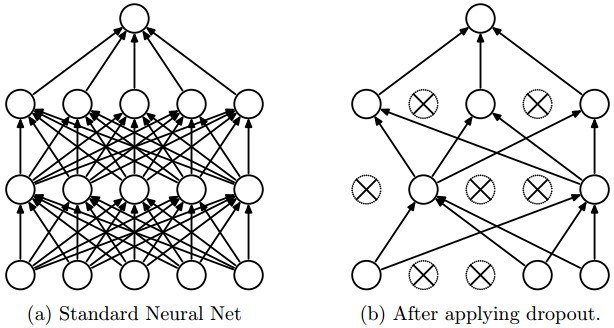
\includegraphics[width=0.5\textwidth]{Images/dropout/1.jpeg}
  \caption{Dropout}
\end{figure}
``Randomly set ~\%50 some neurons to zero in the forward pass."  There two ways of understanding why this works:
\begin{itemize}
\item This makes the network unable to relay on a single feature. Thus, forcing it to generate redundant representation. In this way, you will be representing an object with redundant descriptors, detectors, etc. So in test time, if some features can not be detected, you still can really on the other ones.

\begin{figure}[!htb]
  \centering
  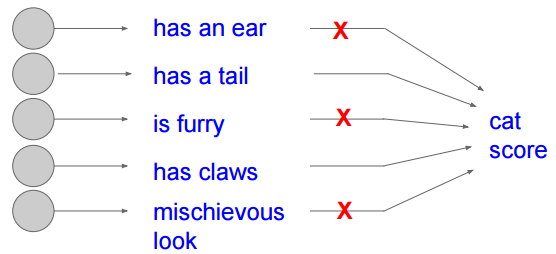
\includegraphics[width=0.45\textwidth]{Images/dropout/3.png}
  \caption{Relay on multiple features}
\end{figure}

\item It can also be seen as training a large ensemble of models that share parameters. When applying a mask to shutdown some randomly neurons at the forward pass this mask stays there for the backward pass. Thus, in the backprop step, no gradient will flow through the neurons that were shut off to zero; so its weights to the previous layer will not be updated. In other words, the neurons that were dropout do not update their connections to the previous layer, just as if they were not there. With dropout you are subsampeling a part of your neural network and training it with the current example. So each binary mask is one model which gets trained on only ~one datapoint (or more in the case that two random mask are equal during training).
\end{itemize}

\textbf{WARNING}: If dropout is not working for you, you should probably be using a bigger network.

\subsection*{Train time}
During the forward pass set ~50\% of the neurons to 0. To get an idea the code below shows a naive implementation of dropout 
\begin{lstlisting}[frame=single] 
""" Vanilla Dropout: Not recommended implementation (see notes below) """

p = 0.5 # probability of keeping a unit active. higher = less dropout

def train_step(X):
  """ X contains the data """

  # forward pass for example 3-layer neural network
  H1 = np.maximum(0, np.dot(W1, X) + b1)
  U1 = np.random.rand(*H1.shape) < p # first dropout mask
  H1 *= U1 # drop!
  H2 = np.maximum(0, np.dot(W2, H1) + b2)
  U2 = np.random.rand(*H2.shape) < p # second dropout mask
  H2 *= U2 # drop!
  out = np.dot(W3, H2) + b3

  # backward pass: compute gradients... (not shown)
  # perform parameter update... (not shown)
 \end{lstlisting}

\subsection*{Test time}
At test time ideally we would like to integrate out all the noise (not possible). A Monte Carlo approximation would be: do many forward passes with different dropout masks, average all predictions. Unfortunately its not time efficient. Instead, you can approximate this method without not droping out any unit in the forward pass during testing but we have to be careful. 

\subsubsection*{Example}
\begin{figure}[!htb]
  \centering
  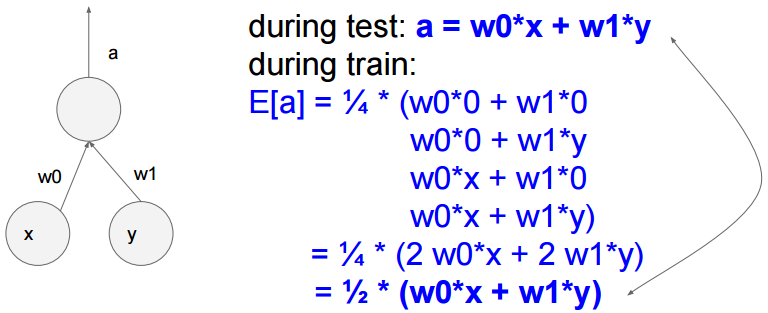
\includegraphics[width=0.45\textwidth]{Images/dropout/2.png}
  \caption{Example}
\end{figure}
Imagine this linear NN and a dropout $prob = 0.5$. During training time the expected value is the average between all the possible masks activation value. However, if we use all the neurons in test time, the activation value is going to be twice the expected value in train time. So it is easy to see that this half comes from the fact that at train time we dropout neurons with probability 50\%.

With $p=0.5$ dropout prob, using all inputs in the forward pass would inflate the activations by $2x$ from what the network was "used to" during training. Thus, you have to compensate by scaling the activations back down by $1/2$. In this way, the ouput at test time is equal to the expected output at training time. Let's see a naive implementation:
\begin{lstlisting}[frame=single] 
""" Vanilla Dropout: Not recommended implementation (see notes below) """

p = 0.5 # probability of keeping a unit active. higher = less dropout

def predict(X):
  # ensembled forward pass
  H1 = np.maximum(0, np.dot(W1, X) + b1) * p # NOTE: scale the activations
  H2 = np.maximum(0, np.dot(W2, H1) + b2) * p # NOTE: scale the activations
  out = np.dot(W3, H2) + b3
\end{lstlisting}

A better way of implementing dropout is using "inverted dropout". The idea is very simple, instead of multiplying the activation values by the dropout probability during test time, divide the training activation values by the dropout probability during train time.  In this way, test time is unchanged.

\begin{lstlisting}[frame=single]
"""
Inverted Dropout: Recommended implementation example.
We drop and scale at train time and don't do anything at test time.
"""

p = 0.5 # probability of keeping a unit active. higher = less dropout

def train_step(X):
  # forward pass for example 3-layer neural network
  H1 = np.maximum(0, np.dot(W1, X) + b1)
  U1 = (np.random.rand(*H1.shape) < p) / p # first dropout mask. Notice /p!
  H1 *= U1 # drop!
  H2 = np.maximum(0, np.dot(W2, H1) + b2)
  U2 = (np.random.rand(*H2.shape) < p) / p # second dropout mask. Notice /p!
  H2 *= U2 # drop!
  out = np.dot(W3, H2) + b3

  # backward pass: compute gradients... (not shown)
  # perform parameter update... (not shown)

def predict(X):
  # ensembled forward pass
  H1 = np.maximum(0, np.dot(W1, X) + b1) # no scaling necessary
  H2 = np.maximum(0, np.dot(W2, H1) + b2)
  out = np.dot(W3, H2) + b3
\end{lstlisting}

There is a method to dropout single weights instead of full neurons call dropconnect